\section{Le schéma}
\begin{figure}[H]
    \centering
    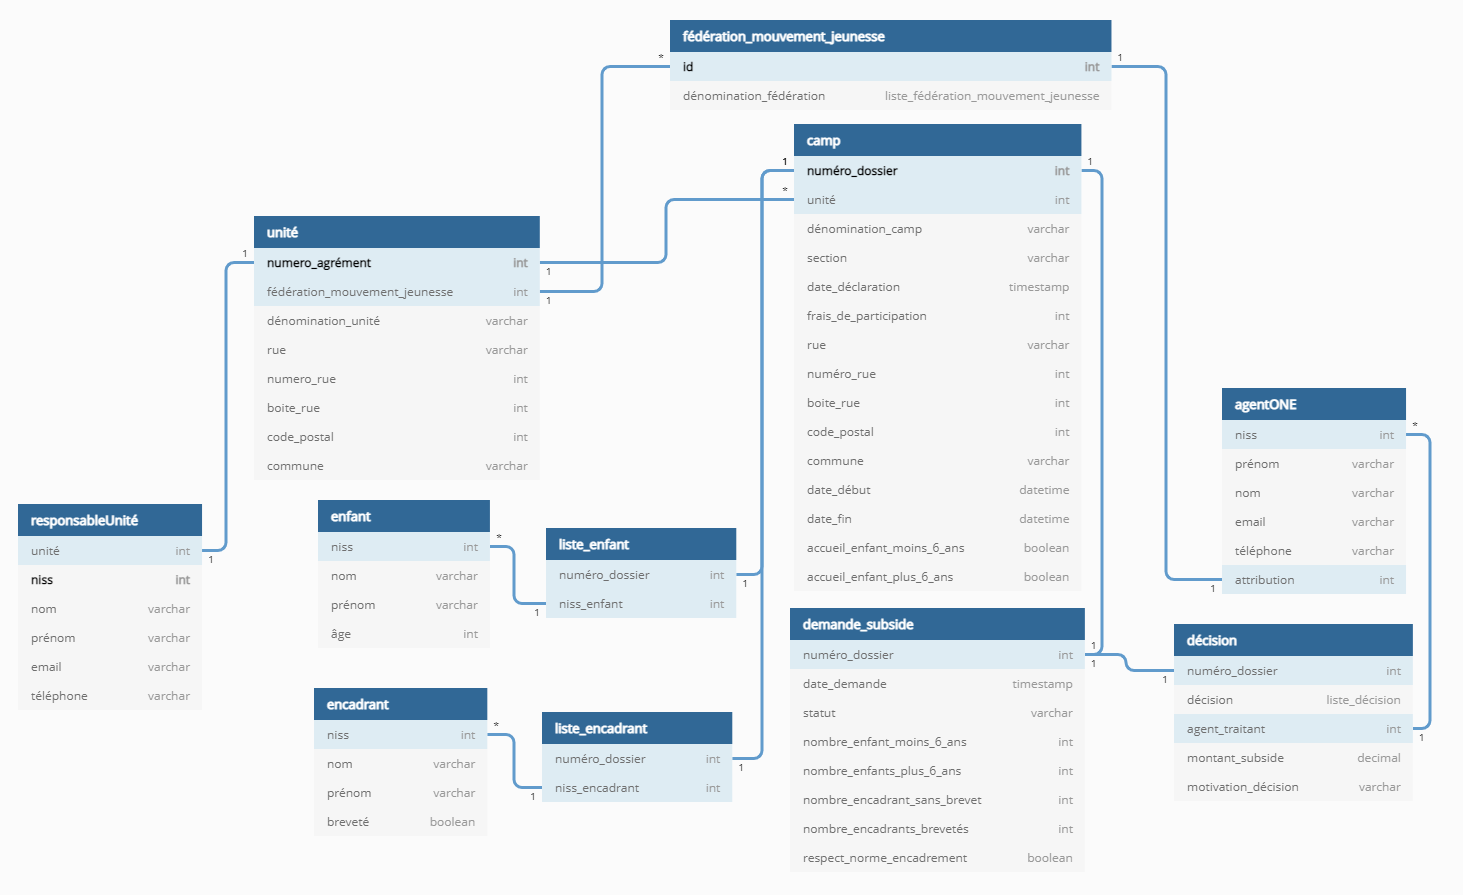
\includegraphics[width=17cm]{Pictures/modele_lr.png}
    \caption{Schéma logique relationnel}
    \label{fig:modele_lr}
\end{figure}


\section{Explication du schéma}
\subsection{Traduction de l'héritage}
Dans la mesure où les personnes ne peuvent avoir le rôle d'encadrants, d'enfants, de responsable d'unité ou agent ONE, qui correspond à une relation totale et exclusive, nous avons opté pour conserver les sous-entités. 

Chaque sous-entités reçoivent donc les attributs de la super-entité.


\subsection{Traduction de certaines associations et contraintes qui en découlent}
\subsubsection{Attribution des agents ONE: gestionnaire de dossiers}
Chaque agent ONE possède une attribution qui lui est propre. Cette attribution est liée à la fédération de mouvement de jeunesse dont il a la charge des dossiers.
\subsubsection{Résolution des cas de many to many pour les listes enfants et encadrants}
Les enfants et les encadrants peuvent participer à plusieurs camps durant une même année. Afin de prévoir ce cas de figure, deux tables viennent compléter le schéma afin d'établir des relations entre participants à de multiples camps. Un attribut année à également été ajouté afin de faciliter les manipulations de données.

\subsection{Choix de ne pas historiser le responsable d'unité}
Concernant la possibilité d'avoir un historique des responsables d'unité, il nous ne nous a pas jugé nécessaire d'ajouter cette dimension. Nous aurions pu résoudre ce cas en créant une entité "mandat" avec l'identité du responsable de projet et l'année concerné.

Seulement, l'ONE conserve les courriers officiels avec le destinataire et son adresse (archivage comptable). Nous saurions par ce biais qui s'occupait dès lors de l'envoie des déclarations et des demandes de subsides.

Cette informations aurait pu servir pour les unités (une base de données de ses membres et de ses mandataires à l'année), mais ne soulève pas un besoin dans notre cas d'application. En effet, si le responsable de projet venait à changer en cours d'année, il est plus utile d'envoyer et de contacter son successeur. 


%titre repris telle quelle des consignes